%%%%%%%%%%%%%%%%%%%%%%%%%%%%%%%%%%%%%%%%%%%%%%%%%%%%%
%%% Task 3 %%%%%%%%%%%%%%%%%%%%%%%%%%%%%%%%%%%%%%%%%%
%%%%%%%%%%%%%%%%%%%%%%%%%%%%%%%%%%%%%%%%%%%%%%%%%%%%%
\task{Line-commuted three-phase rectifier}

%%%%%%%%%%%%%%%%%%%%%%%%%%%%%%%%%%%%%%%%%%%%%%
\taskGerman{Netzgeführter dreiphasiger Gleichrichter}

An industrial conveyor system is powered by a DC motor that is supplied via a controlled three-phase 
midpoint rectifier (M3C). The motor draws a steady current $I_\mathrm{2}$ and operates at a nominal induced  
motor voltage $U_\mathrm{mot,ind}$. The motor has an internal armature resistance $R$. To smooth the output
current, a large inductor ($L \to  \infty$) is placed such that CCM is 
maintained. The input to the rectifier is a symmetrical three-phase grid connected via an ideal 
transformer. On the secondary side, each phase has an effective voltage of 
$U_\mathrm{1,i} = \SI{200}{\volt}$, $\forall i=\mathrm{a, b, c}$. All components (switches, transformer, 
etc.) are ideal.\\
\color{gray}
Ein industrielles Fördersystem wird von einem Gleichstrommotor angetrieben, der über einen geregelten 
Dreiphasen-Mittelpunktgleichrichter (M3C) versorgt wird. Der Motor zieht einen konstanten Strom 
$I_\mathrm{2}$ und weist eine induzierte Spannung $U_\mathrm{mot,ind}$ im Nennpunkt auf. Der Motor hat einen internen 
Ankerwiderstand $R$. Um den Ausgangsstrom zu glätten, wird eine große Induktivität ($L \to  \infty$) so 
platziert, dass der CCM aufrechterhalten bleibt. Der Eingang des Gleichrichters 
ist ein symmetrisches Dreiphasennetz, das über einen idealen Transformator angeschlossen ist. Auf
der Sekundärseite hat jede Phase eine effektive Spannung von $U_\mathrm{1,i} = \SI{200}{\volt}$, 
$\forall i=\mathrm{a, b, c}$. Alle Komponenten (Schalter, Transformator usw.) sind ideal.

\color{black}
%%%%%%%%%%%%%%%%%%%%%%%%%%%%%%%%%%%%%%%%%%%%%%%%%%%%%%%%%%%%%%%%%%%%%%%
 % M3C rectifier with RL Load
%%%%%%%%%%%%%%%%%%%%%%%%%%%%%%%%%%%%%%%%%%%%%%%%%%%%%%%%%%%%%%%%%%%%%%%
\begin{figure}[htb]
  \begin{center}
    \begin{circuitikz}[european currents,european resistors,american inductors]
      \def\vd{1cm} % vertical distance inductors
      \def\htraf{0.75cm} % horizontal distance transformer coils
      \draw (0,0) to [short, o-] ++(0.5,0) coordinate (L1astart) to [short] ++(0.5,0) to [L] ++(2,0) coordinate (L1aend)
      (0,-1*\vd) to [short, o-] ++(1,0) coordinate (L1bstart) to [L] ++(2,0) coordinate (L1bend)
      (0,-2*\vd) to [short, o-] ++(1,0) coordinate (L1cstart) to [L] ++(2,0) coordinate (L1cend) -- ++(0,-0.5*\vd) to (\tikztostart -| L1astart) 
      to [crossing] ++(0, 1*\vd) to [crossing] ++(0, 1*\vd) to [short, -*] (L1astart)
      (L1aend) -- ++(0,-0.5*\vd) to (\tikztostart -| L1bstart) to [short, -*] (L1bstart)
      (L1bend) -- ++(0,-0.5*\vd) to (\tikztostart -| L1cstart) to [short, -*] (L1cstart);
      \draw let \p1=(L1aend) in (\x1 + \htraf, \y1) coordinate (L2astart) to [L, v^<=$u_{1\mathrm{a}}(t)$, voltage = straight] ++(2,0) to [short, i=$i_{1\mathrm{a}}(t)$] ++(0.5,0) coordinate (L2aend);
      \draw let \p1=(L1bend) in (\x1 + \htraf, \y1) coordinate (L2bstart) to [L, v^<=$u_{1\mathrm{b}}(t)$, voltage = straight] ++(2,0) to [short, i=$i_{1\mathrm{b}}(t)$] ++(0.5,0) coordinate (L2bend);
      \draw let \p1=(L1cend) in (\x1 + \htraf, \y1) coordinate (L2cstart) to [L, v^<=$u_{1\mathrm{c}}(t)$, voltage = straight] ++(2,0) to [short, i=$i_{1\mathrm{c}}(t)$] ++(0.5,0)  coordinate (L2cend);
      \draw (L2astart) to [short, -*] (L2bstart) to [short, -*] (L2cstart) -- ++(0, -1.5*\vd) -- ++(9.25,0) coordinate (ui-);
      \draw[double, double distance=3pt, thick] let \p1=(L1aend), \p2=(L2cstart) in (\x1/2+\x2/2, \y1) -- (\x1/2+\x2/2, \y2);
      \draw (L2aend) to [thyristor] ++(2,0) coordinate (D1end);
      \draw (L2bend) to [thyristor] ++(2,0) coordinate (D2end);
      \draw (L2cend) to [thyristor] ++(2,0) coordinate (D3end) to [short, -*] (D2end) to [short, -*] (D1end);
      \draw (D1end) to [short] ++(0.5,0) coordinate (u2) to [short, i=$i_2(t)$] ++(0.75,0) to [L, l=$L$] ++(2,0) coordinate (Ctop) to [short] ++(1.5,0) to node[elmech](motor){M} (ui-);
      %[R, l=$R$] ++(0,-2) coordinate (Rend) to
      
      \draw (u2) to [open, v^>=\hspace{1em}$u_2(t)$, voltage = straight] ++(0,-3.5);
    \end{circuitikz}%
  \end{center}
  \caption{M3C rectifier used for driving a DC motor.}
  \label{fig:M3C_topology_RL_no_filter}
\end{figure}
\begin{table}[ht]
    \centering  % Zentriert die Tabelle
    \begin{tabular}{ll}
        \toprule
        Input voltages ($i=\mathrm{a,b,c}$): & $U_{\mathrm{1},i}=\SI{200}{\volt}$ (phase voltage) \\
                        & $U_{\mathrm{1,LL},i} = \SI{346}{\volt}$ (line-to-line voltage)\\
        Nom. motor current: & $I_{\mathrm{2}} = \SI{50}{\ampere}$ \\
        Nom. motor induced voltage: & $U_\mathrm{mot,ind} = \SI{150}{\volt}$ \\ 
        Motor internal resistance: & $R_\mathrm{mot} = \SI{0.2}{\ohm}$\\ 
        Grid frequency: & $f= \SI{50}{\hertz}$ \\ 
        \bottomrule
    \end{tabular}
    \caption{Drive parameters}  
    \label{table:Task03_ParametersOfTheCircuit}
\end{table}

\subtask{ Calculate the required firing angle $\alpha$ to deliver the specified motor terminal voltage (induced + ohmic). 
Draw the output voltage signal $u_2(t)$ for this angle into \autoref{fig:Task03_M3C_with_RLE}.}{3}
\subtaskGerman{Berechnen Sie den erforderlichen Zündwinkel $\alpha$, um die spezifiziert 
Motoranschlussspannung (induziert + resistiv) zu liefern. Zeichnen Sie der Ausgangsspannung $u_2(t)$ 
für diesen Winkel in \autoref{fig:Task03_M3C_with_RLE}.}
%%%%%%%%%%%%%%%%%%%%%%%%%%%%%%%%%%%%%%%%%%%%%%%%%%%%%%%%%%%%%%%%%%%%%%%%%%
% Output voltage u2 for M3C with RLE-Load
%%%%%%%%%%%%%%%%%%%%%%%%%%%%%%%%%%%%%%%%%%%%%%%%%%%%%%%%%%%%%%%%%%%%%%%%%%
\begin{figure}[htb]
    %   \documentclass{standalone}
    %   \usepackage{pgfplots}
    %   \pgfplotsset{compat=1.18} % Kompatibilität für neuere Versionen
           \centering
           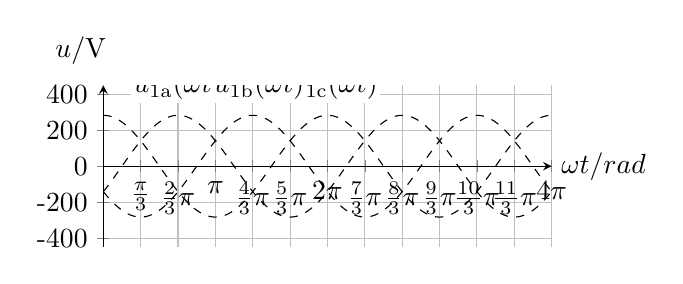
\begin{tikzpicture}
               \begin{axis}[
                   % x/y range adjustment
                   xmin=0, xmax=720,
                   ymin=-450, ymax=450,
                   samples=500,
                   axis y line=center,
                   axis x line=middle,
                   extra y ticks=0,
                   % Label text
                   xlabel={$\omega t / \text{rad}$},,
                   ylabel={$u/\mathrm{V}$},
                   % Label adjustment
                   x label style={at={(axis description cs:1,0.5)},anchor=west},
                   y label style={at={(axis description cs:-.05,.97)},anchor=south,yshift=0.2cm},
                   width=0.6\textwidth,
                   height=0.3\textwidth,
                   % x-Ticks
                   xtick={0,60,120,180,240,300,360, 420, 480, 540, 600, 660, 720},
                   xticklabels={,$\frac{\pi}{3}$,$\frac{2}{3}\pi$,$\pi$, $\frac{4}{3}\pi$,$\frac{5}{3}\pi$,$2\pi$, $\frac{7}{3}\pi$, $\frac{8}{3}\pi$,$\frac{9}{3}\pi$,$\frac{10}{3}\pi$,$\frac{11}{3}\pi$,$4\pi$},
                   xticklabel style = {anchor=north},
                   % y-Ticks
                   ytick={400,200,0,-200,-400},
                   yticklabels={400,200,0,-200,-400},
                   yticklabel style = {anchor=east},
                   % Grid layout
                   grid,
                   %grid style={line width=.1pt, draw=gray!10},
                   %major grid style={line width=.2pt,draw=gray!90},
                     ]
               % Voltage u1a(wt), u1b(wt) u1c(wt)
               \addplot[black, domain= 0:720,dashed] {282.84*cos(x)};
               \addplot[black, domain= 0:720,dashed] {282.84*cos(x+120)};
               \addplot[black, domain= 0:720,dashed] {282.84*cos(x+240)};
               % Label of u1c
               \node[black, fill=white, inner sep = 1pt, anchor = south] at (axis cs:370,350) {$u_{\mathrm{1c}}(\omega t)$}; 
               % Label of u1a
               \node[black, fill=white, inner sep = 1pt, anchor = south] at (axis cs:120,350) {$u_{\mathrm{1a}}(\omega t)$};           
               % Label of u1b
               \node[black, fill=white, inner sep = 1pt, anchor = south] at (axis cs:250,350) {$u_{\mathrm{1b}}(\omega t)$};

           \end{axis}     
           \end{tikzpicture}
           \caption{Output voltage $u_\mathrm{2}(t)$ for $\alpha$.}
           \label{fig:Task03_M3C_with_RLE}
   \end{figure}
\begin{solutionblock}
    First, the voltage drop across the internal resistance can be calculated with
        $$ U_\mathrm{R} = I_2 \cdot R = \SI{50}{\ampere} \cdot \SI{0.2}{\ohm} = \SI{10}{\volt}.$$
        Hence, the required rectifier output voltage is
        $$ \bar{u}_\mathrm{2} =  U_\mathrm{mot,term} = U_\mathrm{mot,ind} + U_\mathrm{R} = \SI{150}{\volt} + \SI{10}{\volt} = \SI{160}{\volt}.$$
        Also, the peak phase voltage is:
        $$ \hat{u}_\mathrm{1} = \sqrt{2} \cdot U_\mathrm{1,i} = \sqrt{2} \cdot \SI{200}{\volt} \approx \SI{282.84}{\volt}.$$
        So, using the average voltage equation of B6C, $\alpha$ can be calculated as 
        $$\SI{160}{\volt} = \frac{3\sqrt{3}}{2\pi} \cdot \SI{282.84}{\volt} \cdot \cos(\alpha)
        \Rightarrow \cos(\alpha) = \frac{\SI{160}{\volt} \cdot 2\pi}{3\sqrt{3} \cdot \SI{282.84}{\volt}}
        \approx 0.684,$$
        $$\alpha = \cos^{-1}(0.684) \approx \SI{46.84}{\degree}.$$
%%%%%%%%%%%%%%%%%%%%%%%%%%%%%%%%%%%%%%%%%%%%%%%%%%%%%%%%%%%%%%%%%%%%%%%%%%
% Output voltage u2 for M3C with RLE-Load
%%%%%%%%%%%%%%%%%%%%%%%%%%%%%%%%%%%%%%%%%%%%%%%%%%%%%%%%%%%%%%%%%%%%%%%%%%
\begin{solutionfigure}[htb]
    %   \documentclass{standalone}
    %   \usepackage{pgfplots}
    %   \pgfplotsset{compat=1.18} % Kompatibilität für neuere Versionen
           \centering
           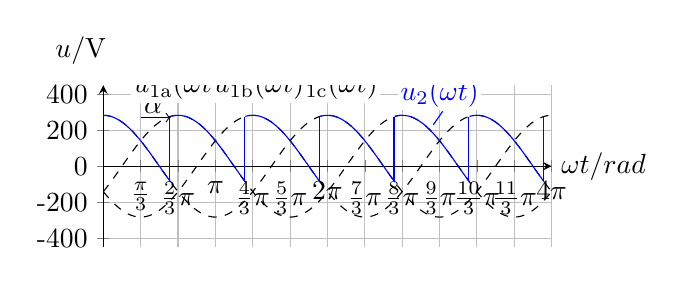
\begin{tikzpicture}
               \begin{axis}[
                   % x/y range adjustment
                   xmin=0, xmax=720,
                   ymin=-450, ymax=450,
                   samples=500,
                   axis y line=center,
                   axis x line=middle,
                   extra y ticks=0,
                   % Label text
                   xlabel={$\omega t / \text{rad}$},,
                   ylabel={$u/\mathrm{V}$},
                   % Label adjustment
                   x label style={at={(axis description cs:1,0.5)},anchor=west},
                   y label style={at={(axis description cs:-.05,.97)},anchor=south,yshift=0.2cm},
                   width=0.6\textwidth,
                   height=0.3\textwidth,
                   % x-Ticks
                   xtick={0,60,120,180,240,300,360, 420, 480, 540, 600, 660, 720},
                   xticklabels={,$\frac{\pi}{3}$,$\frac{2}{3}\pi$,$\pi$, $\frac{4}{3}\pi$,$\frac{5}{3}\pi$,$2\pi$, $\frac{7}{3}\pi$, $\frac{8}{3}\pi$,$\frac{9}{3}\pi$,$\frac{10}{3}\pi$,$\frac{11}{3}\pi$,$4\pi$},
                   xticklabel style = {anchor=north},
                   % y-Ticks
                   ytick={400,200,0,-200,-400},
                   yticklabels={400,200,0,-200,-400},
                   yticklabel style = {anchor=east},
                   % Grid layout
                   grid,
                   %grid style={line width=.1pt, draw=gray!10},
                   %major grid style={line width=.2pt,draw=gray!90},
                     ]
               % Voltage u1a(wt), u1b(wt) u1c(wt)
               \addplot[black, domain= 0:720,dashed] {282.84 *cos(x)};
               \addplot[black, domain= 0:720,dashed] {282.84 *cos(x+120)};
               \addplot[black, domain= 0:720,dashed] {282.84 *cos(x+240)};
   
               % Voltage u2(wt)
               \addplot[blue, domain= 0:108.17] {282.84 *cos(x)}; 
               \addplot[blue, domain= 108.17:228.17] {282.84 *cos(x+240)};     
               \addplot[blue, domain= 228.17:348.17] {282.84 *cos(x+120)};    
               \addplot[blue, domain= 348.17:468.17] {282.84 *cos(x)};
               \addplot[blue, domain= 468.17:588.17] {282.84 *cos(x+240)}; 
               \addplot[blue, domain= 588.17:708.17] {282.84 *cos(x+120)};
               \addplot[color=blue,solid] coordinates{
                (106.84,-81.94)   %(60+alpha,282.84*cos(60+alpha))
                (106.84, 275.41) %(60+alpha,282.84*cos(60+alpha + 240))
                };               
               \addplot[color=blue,solid] coordinates{
                   (226.84,-81.94)
                   (226.84, 275.41)
                };     
               \addplot[color=blue,solid] coordinates{
                   (346.84,-81.94)
                   (346.84,  275.41)
                };     
               \addplot[color=blue,solid] coordinates{
                   (466.84,-81.94)
                   (466.84, 275.41)
                };
               \addplot[color=blue,solid] coordinates{
                (586.84,-81.94)
                (586.84, 275.41)
                };               
               \addplot[color=blue,solid] coordinates{
                   (706.84,-81.94)
                   (706.84, 275.41)
                };     
                % Label of u2
               \node[blue, fill=white, inner sep = 1pt, anchor = south] at (axis cs:540,310) {$u_{\mathrm{2}}(\omega t)$};
                % Line to u2
               \draw[thin, blue] (545,305) -- (530,230);
                %Label alpha
               \node[black, fill=white, inner sep = 1pt, anchor = south] at (axis cs:80,275){$\alpha$};
               % Line for alpha
               \draw[->](60,270) -- (108.17,270);
           
               % Label of u1c
               \node[black, fill=white, inner sep = 1pt, anchor = south] at (axis cs:370,350) {$u_{\mathrm{1c}}(\omega t)$}; 
               % Label of u1a
               \node[black, fill=white, inner sep = 1pt, anchor = south] at (axis cs:120,350) {$u_{\mathrm{1a}}(\omega t)$};           
               % Label of u1b
               \node[black, fill=white, inner sep = 1pt, anchor = south] at (axis cs:250,350) {$u_{\mathrm{1b}}(\omega t)$};

           \end{axis}     
           \end{tikzpicture}
           \caption{Output voltage $u_\mathrm{2}(t)$ for $\alpha = 46.84$.}
           \label{sfig:subtask3.1_output_voltage}
   \end{solutionfigure}
\end{solutionblock}
\subtask{Explain how adjusting $\alpha$ affects the speed of the motor, especially $\alpha = 
\frac{\pi}{2}$ and $\alpha = 0$.}{3}
\begin{hintblock}
    the motors' speed is proportional to the back EMF ($ \omega \propto U_\mathrm{mot,ind} $).
\end{hintblock}
\subtaskGerman{Erklären Sie, wie sich die Einstellung von $\alpha$ auf die Drehzahl des Gleichstrommotors 
auswirkt, insbesondere $\alpha = \frac{\pi}{2}$ and $\alpha = 0$.}

\begin{germanhintblock}
    die Drehzahl der Motoren ist proportional zur Gegen-EMK ($ \omega \propto U_\mathrm{mot,ind} $).
\end{germanhintblock}
\begin{solutionblock}
The average voltage applied to the motor is controlled by the firing angle $\alpha $. The motor speed 
$\omega $ (assuming constant flux and neglecting armature reaction) is approximately proportional to the 
back EMF $U_\mathrm{mot,ind}$, which is itself proportional to the applied voltage minus internal resistance drop:
$$ U_\mathrm{mot,ind} = \bar{u}_\mathrm{2} - I_\mathrm{2} R_\mathrm{internal}.$$
Since:
$$ \omega \propto U_\mathrm{mot,ind} \Rightarrow \omega \propto \bar{u}_\mathrm{2} - I_\mathrm{2} R_\mathrm{internal}, $$
and:
$$ \bar{u}_\mathrm{2} = \frac{3\sqrt{2}}{\pi} \hat{u}_\mathrm{1} \cos(\alpha), $$
we conclude:
$$ \omega \propto \cos(\alpha).$$
So increasing $ \alpha $ reduces $ \cos(\alpha) $, leading to lower $\bar{u}_\mathrm{2}$ and thus lower motor 
speed. Conversely, reducing $ \alpha $ increases speed.
\vspace{0.3em}
\textbf{Constraints on $\alpha$:}
\begin{itemize}
    \item $\alpha$ should not be too small (close to $ \SI{0}{\degree} $), as this results in maximum 
    $\bar{u}_\mathrm{2}$ and could lead to overvoltage and overspeed conditions in the motor.
    \item $\alpha$ must be kept below $ 90^\circ $. At $ \alpha = \SI{90}{\degree} $, $ \cos(\alpha) = 0 $, 
    which gives zero output voltage.
\end{itemize}
\end{solutionblock}
\subtask{Calculate the output power delivered to the motor, the power dissipated in the internal 
resistance, and the total power drawn from the rectifier output.}{3}
\subtaskGerman{Berechnen Sie die an den Motor abgegebene Ausgangsleistung, die im Innenwiderstand 
dissipierte Leistung und die vom Gleichrichterausgang insgesamt aufgenommene Leistung.}
\begin{solutionblock}
 \begin{itemize}
        \item Motor power output:
        $$ P_\mathrm{mot,ind} = U_\mathrm{mot,ind} \cdot I_\mathrm{2} = \SI{150}{\volt} \cdot \SI{50}{\ampere} = \SI{7500}{\watt}. $$
        \item Power loss in internal resistance:
        $$ P_\mathrm{R} = I^2_\mathrm{2} \cdot R = \SI{50^2}{\ampere^2} \cdot \SI{0.2}{\ohm} = \SI{500}{\watt}. $$
        \item Total power drawn from rectifier:
        $$ P_\mathrm{total} = \bar{u}_\mathrm{2} \cdot I_\mathrm{2} = \SI{160}{\volt} \cdot \SI{50}{\ampere} = \SI{8000}{\watt}. $$
    \end{itemize}
\end{solutionblock}
\subtask{Sketch the input current $i_\mathrm{1a}(\omega t)$ in \autoref{sfig:task03_current_signal_3_5}, calculate the effective 
value of the fundamental component $I^\mathrm{(1)}_\mathrm{1a}$ and the corresponding total harmonic distortion (THD).}{4}
\begin{hintblock}
    to calculate the THD, use $$ \mathrm{THD} = \sqrt{\left(\frac{I^2_\mathrm{1a}}{(I^\mathrm{(1)}_\mathrm{1a})^2}\right)-1},$$ where $I_\mathrm{1a}$
    is the effective value of the phase current. 
\end{hintblock}
\subtaskGerman{Zeichnen Sie den Eingangsstrom $i_\mathrm{1a}(\omega t)$ in \autoref{sfig:task03_current_signal_3_5}, Berechnen Sie den Effektivwert der Grundkomponente $I^\mathrm{(1)}_\mathrm{1a}$, 
und berechnen Sie die entsprechende gesamte harmonische Verzerrung (THD).}
\begin{germanhintblock}
    um den THD zu berechnen, verwenden Sie die obige Gleichung, wobei $I_\mathrm{1a}$ der effektive Wert des Phasenstroms ist.
\end{germanhintblock}
 \input{fig/Task03/Fig_subtask3.4.tex}
\begin{solutionblock}
 %%%%%%%%%%%%%%%%%%%%%%%%%%%%%%%%%%%%%%%%%%%%%%%%%%%%%%%%%%%%%%%%%%%%%%%%%%
% Current i_1a(wt)
%%%%%%%%%%%%%%%%%%%%%%%%%%%%%%%%%%%%%%%%%%%%%%%%%%%%%%%%%%%%%%%%%%%%%%%%%%
\begin{solutionfigure}[htb]

    %   \documentclass{standalone}
    %   \usepackage{pgfplots}
    %   \pgfplotsset{compat=1.18} % Kompatibilität für neuere Versionen
           \centering
           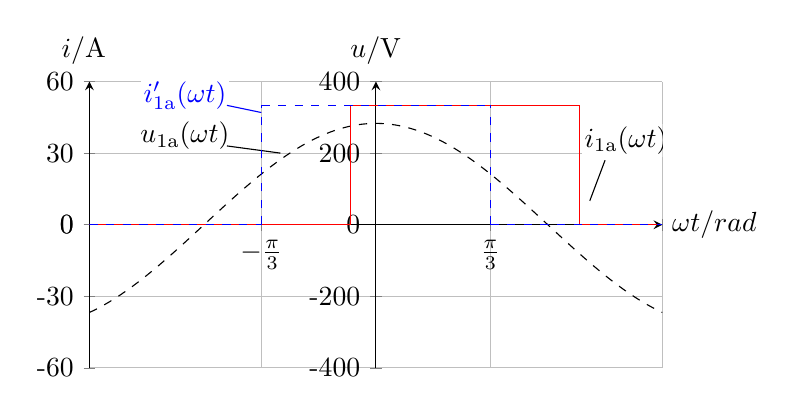
\begin{tikzpicture}
                \pgfplotsset{set layers}
               \begin{axis}[
                   % x/y range adjustment
                   scale only axis,
                   xmin=-150, xmax=150,
                   ymin=-40, ymax=40,
                   samples=500,
                   axis y line=center,
                   axis x line=middle,
                   extra y ticks=0,
                   % Label text
                   xlabel={$\omega t / \text{rad}$},
                   ylabel={$u/\mathrm{V}$},
                   % Label adjustment
                   x label style={at={(axis description cs:1,0.5)},anchor=west},
                   y label style={at={(axis description cs:0.5,.97)},anchor=south,yshift=0.2cm},
                   width=0.6\textwidth,
                   height=0.3\textwidth,
                   % x-Ticks
                   xtick={-150,-60,0,60,150},
                   xticklabels={,$-\frac{\pi}{3}$,0,$\frac{\pi}{3}$,,},
                   xticklabel style = {anchor=north},
                   % y-Ticks
                   ytick={40,20,0,-20,-40},
                   yticklabels={400,200,0,-200,-400},
                   yticklabel style = {anchor=east},
                   % Grid layout
                   grid,
                   %grid style={line width=.1pt, draw=gray!10},
                   %major grid style={line width=.2pt,draw=gray!90},
               ]
               % Voltage u1a(wt)
               \addplot[black, domain= -150:150,dashed] {28.3*cos(x)};
                
                % Label of u1a           
               \node[black, fill=white, inner sep = 1pt, anchor = south] at (axis cs:-100,20) {$u_{\mathrm{1a}}(\omega t)$}; 
               % Line for u1a
               \draw[thin, black] (-78,22) -- (-50,20);
           
           \end{axis}
           \begin{axis}[
            % x/y range adjustment
            scale only axis,
            ymin=-60, ymax=60,
            xmin=-150, xmax=150,
            axis x line=none, 
            samples=500,
            axis y line=left,
            axis x line=middle,
            extra y ticks=0,
            % Label text
            ylabel={$i/\mathrm{A}$},
            % Label adjustment
            y label style={rotate = -90,at={(axis description cs:-0.01,.97)},anchor=south,yshift=0.2cm},
            width=0.6\textwidth,
            height=0.3\textwidth,
            % y-Ticks
            ytick={60,30,0,-30,-60},
            yticklabels={60,30,0,-30,-60},
            yticklabel style = {anchor=east},
            % Grid layout
            grid,
            %grid style={line width=.1pt, draw=gray!10},
            %major grid style={line width=.2pt,draw=gray!90},
        ] 
        % Current i1a(wt)
        \addplot[color=red,solid] coordinates{
            (-150,0)
            (-13.16, 0)
        };                 
           \addplot[color=red,solid] coordinates{
            (-13.16,0)
            (-13.16, 50)
        };                   
           \addplot[color=red,solid] coordinates{
               (-13.16,50)
               (106.84, 50)
           };  
           \addplot[color=red,solid] coordinates{
            (106.84,0)
            (106.84, 50)
        };
        \addplot[color=red,solid] coordinates{
            (106.84,0)
            (150, 0)
        };
        % Current i1a(wt) modified
        \addplot[color=blue,dashed] coordinates{
            (-150,0)
            (-60, 0)
        };                 
           \addplot[color=blue,dashed] coordinates{
            (-60,0)
            (-60, 50)
        };                   
           \addplot[color=blue,dashed] coordinates{
               (-60,50)
               (60, 50)
           };  
           \addplot[color=blue,dashed] coordinates{
            (60,0)
            (60, 50)
        };
        \addplot[color=blue,dashed] coordinates{
            (60,0)
            (150, 0)
        };    
           % Label of i1a
           \node[black, fill=white, inner sep = 1pt, anchor = south] at (axis cs:131,28) {$i_{\mathrm{1a}}(\omega t)$};
            % Line to i1a
            \draw[thin, black] (112,10) -- (120,27);
            % Label of shifted i1a
           \node[blue, fill=white, inner sep = 1pt, anchor = south] at (axis cs:-100,47) {$i'_{\mathrm{1a}}(\omega t)$};
            % Line to shifted i1a
            \draw[thin, blue] (-78,50) -- (-60,47);
           \end{axis}    
           \end{tikzpicture}
           \caption{Input current $i_\mathrm{1a}(\omega t)$ and $u_\mathrm{1a}(\omega t)$.}
           \label{sfig:task03_current_signals_3_5}
   \end{solutionfigure}

    For simplification, we can position the y-xis in the middle of the conducting period of $i_\mathrm{1a}(\omega t)$ 
    signal and make use of the period's symmetry. This would simplify the calculations by integrating over one 
    half of the period and then multiply by 2. 
    One can see that the shifted signal $i'_{\mathrm{1a}}(\omega t)$ is an even signal, hence, we expect that the fundamental component of the Fourier 
    Series would contain only cosine component ($a_1 \neq 0$) and no sine component ($b_1 = 0$). 
        
     In this case the integration would be from 0 to $\frac{\pi}{3}$, as 
    one conducting period is equal to $\frac{2\pi}{3}$. Thus, $a_1$ ($\hat{i}^\mathrm{(1)}_\mathrm{1a}$) 
    can be calculated as:

        
    $$ a_1 = \hat{i}^\mathrm{(1)}_\mathrm{1a} = \frac{2}{\pi}\int_{0}^{\frac{\pi}{3}}I_\mathrm{2}\cos(\omega t) \mathrm{d}\omega t = \left[\frac{2}{\pi} I_\mathrm{2} \sin(\omega t)\right]^{\frac{\pi}{3}}_{0} = \frac{1}{\pi}I_\mathrm{2}\sqrt{3}.$$  
        
    Then the effective value $I^\mathrm{(1)}_\mathrm{1a}$ is
    
    $$ I^\mathrm{(1)}_\mathrm{1a} = \frac{\hat{i}^\mathrm{(1)}_\mathrm{1a}}{\sqrt{2}} \approx \SI{19.49}{\ampere}.$$
        
    Moreover, the effective value of $I_\mathrm{1a}$ can be calculated as 
    
    $$ I_\mathrm{1a} = \sqrt{\frac{1}{2\pi}\int_{0}^{\frac{2\pi}{3}} I^2_\mathrm{2}\mathrm{d}\omega t} =  \frac{I_\mathrm{2}}{\sqrt{3}} \approx \SI{28.87}{\ampere}.$$   
    So, the THD is
    
    $$ \mathrm{THD} = \sqrt{\left(\frac{I^2_\mathrm{1a}}{(I^\mathrm{(1)}_\mathrm{1a})^2}\right)-1} = \SI{109.3}{\percent}.$$ 
\end{solutionblock}
\subtask{Suppose the inductance of the inductor is finite and was designed too low. How 
would that affect the output voltage and current?}{2}

\subtaskGerman{ Angenommen die Induktivität der Glättungsdrossel habe einen endlichen und zu niedrigen Wert. 
Wie würde sich das auf die Ausgangsspannung und den Ausgangsstrom auswirken?}

\begin{solutionblock}
If the inductance is finite, it cannot sustain continuous current when the AC voltage drops below the DC output voltage. 
The current reaches zero before the next thyristor is triggered. This causes the load current to fall to zero during part of
the cycle, discontinuity in load current.
\end{solutionblock}